\documentclass[a4paper, 10pt]{article}
\usepackage[utf8x]{inputenc}
\usepackage{graphicx}
\usepackage{geometry}
\usepackage{amsmath}
\usepackage{mathenv}
\usepackage{amssymb}
\usepackage{amsfonts}
\usepackage{mathrsfs}
\usepackage{textcomp}
\usepackage{subfigure}
\usepackage{graphics}
\usepackage{pstricks,pstricks-add,pst-math,pst-xkey}
\usepackage{multicol}
\geometry{hmargin = 2.5cm, vmargin = 1.5cm}

% OPENING
\title{SY19 - TP01\\Positionnement multidimensionnel}
\author{Alice Ngwembou - Antoine Hars}

\begin{document}

\maketitle

\section*{Exercice 1 : Exercice théorique}
\subsection*{Première partie : ACP}
% QUESTION 1.1
\textbf{Question 1 :}\\
Afin de calculer les axes factoriels de l'ACP du nuage de points définis, nous centrons, dans un premier temps, la matrice donnée,
ce qui nous permet de prendre comme nouvele origine le centre de gravité dans l'espace des individus.\\
Nous calculons ensuite la matrice de covariance \textit{S} pour appliquer la fonction \textit{eigen()} sur cette dernière,
ce qui nous donne les résultats suivants :\\ \\
\begin{tabular}{|c|c|c|c|c|c|c|c|c|}
\hline
 & $\lambda1$ & $\lambda2$ & $\lambda3$ & $\lambda4$ & $\lambda5$ & $\lambda6$ & $\lambda7$ & $\lambda8$ \\
\hline
Valeurs propres & 24.26 & 0.006 & 3.85e-16 & 3.65e-17 & 1.52e-19 & -1.84e-19 & -7.17e-16 & -1.50e-15 \\
\hline
Inerties expliquées & 98.45\% & 100\% & 100\% & 100\% & 100\% & 100\% & 100\% & 100\% \\
\hline
\end{tabular}\\
\textit{Tableau des valeurs propres et obtenues sur le nuage de points définis.}\\ \\
D'après les valeurs obtenues, nous pouvons dire que seules les 2 premières valeurs de valeur propres sont intéressantes car les valeurs
suivantes sont excessivement proches de zéro (positives ou négatives) mais nous veillons à calculer les inerties expliqués en nous
basant sur la somme des valeurs absolues des valeurs propres.\\
Nous pouvons donc remarquer que les 2 premiers axes factoriels, donc le plan factoriel défini par ces 2 axes,
cumulent environ 100\% de l'information.\\ \\
% QUESTION 1.2
\textbf{Question 2 :}\\
La matrice de composantes principales nous permettent de représenter les 8 individus dans le premier plan factoriel :\\
% TODO : Mettre côte à côte la matrice et le graphique.
$C = X * M * U = \begin{pmatrix} -3.62 & 0.60 \\ 2.47 & 0.29 \\ 4.54 & -0.18 \\ -4.47 & 0.07 \\
-3.09 & -0.24 \\ 3.69 & -0.71 \\ -3.52 & -0.51 \\ 4.01 & 0.67 \end{pmatrix}$\\      
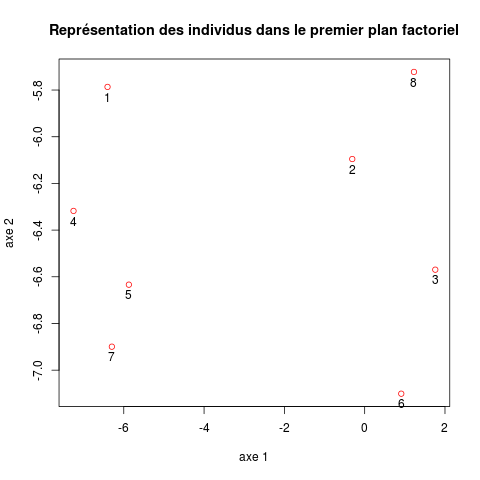
\includegraphics[height = 7cm, width = 7cm]{plots/biplot_exo1_princomp.png}\\
L'ACP applique un changement de base au jeu de données car on a cherché à obtenir une représentation fidèle du nuage de points en
le projetant sur un espace de plus faible dimension (dans notre cas, de dimension 2) sans perdre trop d'informations.
Les variables obtenues par la projection sont donc des combinaisons linéaires des variables du nuage initial.\\ \\
% QUESTION 1.3
\textbf{Question 3 :}\\
$\varSigma^{k}_{\alpha=1} c_{\alpha}u_{\alpha}'$ pour \textit{k = 1} et \textit{k = 2} nous permet de retrouver notre matrice X de départ,
à savoir la matrice contenant le jeu de données : $X = \varSigma^{k}_{\alpha=1} c_{\alpha}u_{\alpha}'$.

\subsection*{Deuxième partie : MDS}
% QUESTION 2.1
\textbf{Question 1 :}\\


\section*{Exercice 3 : Les données de distances entre aéroports}
Dans cet exercice, nous avons travaillé sur les données contenues dans le fichier \textit{airport2.txt} qui représentent les distances de vol
entre des aéroports situés dans le monde. L'objectif de cet exercice était d'appliquer les différentes méthodes
de positionnement multidimensionnel à ces données et de comparer les résultats obtenus.\\ \\
% Question 1
\textbf{Réalisation de l'AFTD sur les données avec \textit{cmdscale} et analyse des résultats obtenus.}\\
L'exécution de la fonction \textit{cmdscale} sur le tableau de distance des données nous a donné le graphique suivant :\\
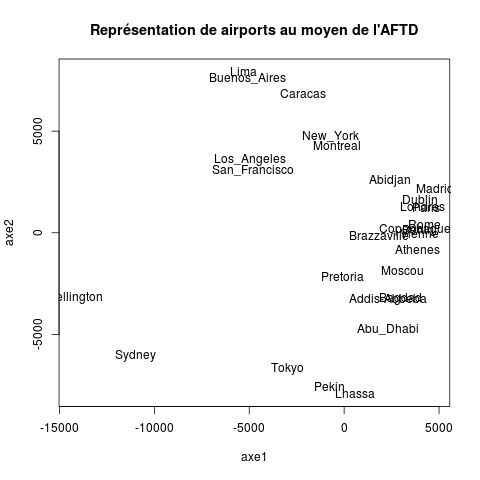
\includegraphics[height = 8cm, width = 8cm]{plots/plot_airports_cmdscale.png}\\

\end{document}
